\begin{figure}[t]
    \centering
    \makebox[\textwidth][c]{
    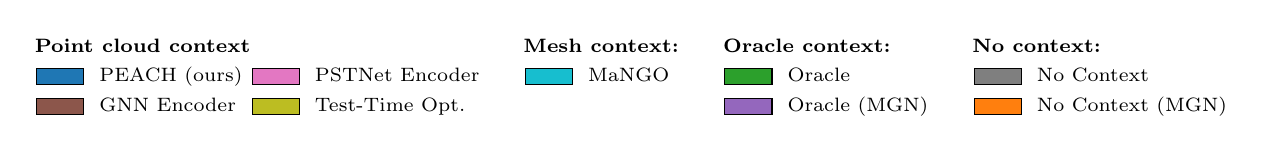
\begin{tikzpicture}
    \tikzstyle{every node}=[font=\scriptsize]
    \definecolor{tabblue}{RGB}{31, 119, 180}
\definecolor{taborange}{RGB}{255, 127, 14}
\definecolor{tabgreen}{RGB}{44, 160, 44}
\definecolor{tabred}{RGB}{214, 39, 40}
\definecolor{tabpurple}{RGB}{148, 103, 189}
\definecolor{tabbrown}{RGB}{140, 86, 75}
\definecolor{tabpink}{RGB}{227, 119, 194}
\definecolor{tabgray}{RGB}{127, 127, 127}
\definecolor{tabolive}{RGB}{188, 189, 34}
\definecolor{tabcyan}{RGB}{23, 190, 207}
\definecolor{ForestGreen}{RGB}{34, 139, 34}
    \begin{axis}[%
        hide axis,
        xmin=10,
        xmax=50,
        ymin=0,
        ymax=0.1,
        legend style={
            draw=none,
            legend cell align=left,
            legend columns=8,
            column sep=0.8ex,
            % smaller gap between the two point cloud columns
            /tikz/column 2/.style={column sep=0.3ex},
        }
    ]
    % ---------------- Row 1: group headers ----------------
    \addlegendimage{area legend, fill=white, draw=white, line width=0pt}
    \addlegendentry{\rlap{\hspace{-8.2mm}\textbf{Point cloud context:}}}
    \addlegendimage{area legend, fill=white, draw=white, line width=0pt}
    \addlegendentry{}
    % spacer
    \addlegendimage{empty legend}
    \addlegendentry{\hspace{1ex}}
    \addlegendimage{area legend, fill=white, draw=white, line width=0pt}
    \addlegendentry{\hspace{-8.2mm}\textbf{Mesh context:}}
    % spacer
    \addlegendimage{empty legend}
    \addlegendentry{\hspace{1ex}}
    \addlegendimage{area legend, fill=white, draw=white, line width=0pt}
    \addlegendentry{\hspace{-8.2mm}\textbf{Oracle context:}}
    % spacer
    \addlegendimage{empty legend}
    \addlegendentry{\hspace{1ex}}
    \addlegendimage{area legend, fill=white, draw=white, line width=0pt}
    \addlegendentry{\hspace{-8.2mm}\textbf{No context:}}

    % ---------------- Row 2 ----------------
    \addlegendimage{area legend, fill=tabblue}
    \addlegendentry{PEACH (ours)}
    \addlegendimage{area legend, fill=tabpink}
    \addlegendentry{PSTNet Encoder}
    % spacer
    \addlegendimage{empty legend}
    \addlegendentry{}
    \addlegendimage{area legend, fill=tabcyan}
    \addlegendentry{MaNGO}
    % spacer
    \addlegendimage{empty legend}
    \addlegendentry{}
    \addlegendimage{area legend, fill=tabgreen}
    \addlegendentry{Oracle}
    % spacer
    \addlegendimage{empty legend}
    \addlegendentry{}
    \addlegendimage{area legend, fill=tabgray}
    \addlegendentry{No Context}

    % ---------------- Row 3 ----------------
    \addlegendimage{area legend, fill=tabbrown}
    \addlegendentry{GNN Encoder}
    \addlegendimage{area legend, fill=tabolive}
    \addlegendentry{Test-Time Opt.}
    % spacer
    \addlegendimage{empty legend}
    \addlegendentry{}
    % empty cell below MaNGO
    \addlegendimage{area legend, fill=white, draw=white, line width=0pt}
    \addlegendentry{}
    % spacer
    \addlegendimage{empty legend}
    \addlegendentry{}
    \addlegendimage{area legend, fill=tabpurple}
    \addlegendentry{Oracle (MGN)}
    % spacer
    \addlegendimage{empty legend}
    \addlegendentry{}
    \addlegendimage{area legend, fill=taborange}
    \addlegendentry{No Context (MGN)}
    \end{axis}
\end{tikzpicture}
    }
    \includegraphics[width=0.24\textwidth]{figures/quantitative_results/db/db_ml_loss.pdf}
    \includegraphics[width=0.24\textwidth]{figures/quantitative_results/db/db_mat_prop_loss.pdf}
    \includegraphics[width=0.24\textwidth]{figures/quantitative_results/sd/sd_ml_loss.pdf}
    \includegraphics[width=0.24\textwidth]{figures/quantitative_results/sd/sd_mat_prop_loss.pdf}
    \caption{
    Full simulation rollout and material property \gls{mse} across different encoder architectures as a function of the number of context sequences for (\textbf{left}) \texttt{Deforming Block} and (\textbf{right}) \texttt{Sheet Deformation}.
    \gls{peach} consistently performs similar to the mesh-based \gls{mango}, improving over other point cloud encoders and achieving near-Oracle performance on \texttt{Deforming Block}.
    }
    \label{fig:quantitative_comparison}
\end{figure}